% !TEX encoding = UTF-8 Unicode
% $Id: 06-hwcentric.tex 36 2018-06-06 08:00:27Z lohmann $

\documentclass{lecturefig}

 \tikzset{
    box/.style={
      rectangle, fill=white,
      minimum height=4ex, minimum width=16em,
      text width=5cm, text badly centered, draw,
      node distance=7ex,
    },
    label position   = left,
    label distance   = 3ex,
		tooldesc/.style={
			box,
			draw=none,
			anchor=west,
			minimum width=5.1cm,
			text width=5.1cm,
			font=\small,
			text ragged,
			inner xsep=1ex,
		},
    tool/.style={
      rounded corners=5pt, fill=srared!#1!white,
      minimum height=3ex-\pgflinewidth,
      inner sep=1pt,
      minimum width=16ex,
      draw=none,
      opacity=1,
    },
    layerdesc/.style={
      draw,<->, shorten >=0.25ex, shorten <=-1ex,
      font=\footnotesize\itshape,
      every node/.style={rotate=90, fill=#1, inner ysep=0pt},
      transform canvas={xshift=-1.5ex},
    },
		machine/.style={
			draw=luhblue, thick, rounded corners=0.25ex,
			fill=luhblue!10!white,
			fill opacity=0.85,
			text opacity=1,
			text=luhblue,
			font=\bfseries,
			text height=13ex,
			minimum width=9ex,
			visible on=<{3-}>,
			inner ysep=2ex,
		},
		shared/.style={
			draw=luhblue, very thin, rounded corners=0.25ex,
			fill=luhblue!10!white,
			text=black,
			font=\footnotesize\it,
			minimum width=8ex,
			minimum height=3ex,
		},
		lecture/.style={
			rounded corners=0.75ex,
			text=white,
			fill=#1,
			minimum width=3.5cm,
			minimum height=4ex,
		},
		lecture/.default=luhblue,
		sra lecture/.style={
			lecture=srared,
		},
		sra ma lecture/.style={
			sra lecture,
			xshift=0.3cm,
			minimum width=2.9cm,
			minimum height=5.25ex,
			font=\slshape,
		},
  }

\begin{document}

\tikzset{
	pics/.cd,
	nothing/.style={},
	layers/.style={code={%
		\node[box, label=$E_0$] (dle)                 {Logikebene};
		\node[box, label=$E_1$, above of=dle] (mae)   {Mikroarchitekturebene};
		\node[box, label=$E_2$, above of=mae] (bse)   {Befehlssatzebene};
		\node[box, label=$E_3$, above of=bse] (mpe)    {Maschinenprogrammebene};
		\node[box, label=$E_4$, above of=mpe] (ase)    {Assemblersprachenebene};
		\node[box, label=$E_5$, onslide=<2>{fill=luhblue,text=white},above of=ase] (pose)   {Hochsprachenebene};
		\begin{scope}[every node/.style={pos=0.5}]
			\draw (pose.south) to coordinate(HLL) (ase.north);
			\draw (ase.south) to coordinate(SYS) (mpe.north);
			\draw (mpe.south) to coordinate(BS) (bse.north);
			\draw (bse.south) to coordinate(OPS) (mae.north);
			\draw (mae.south) to coordinate(mOPS) (dle.north);
		\end{scope}
		\begin{scope}[on background layer]
			\node[inner sep=1.5ex, fill=black!40, rounded corners=0.75ex, fit=(dle) (mae) (mpe) ($(mpe.north west) + (left:1ex)$)](HW){};
			\node[inner sep=1.5ex, fill=black!20, rounded corners=0.75ex, fit=(ase) ($(pose.north west) + (left:1ex)$)](SW){};
			\coordinate[at=(HW.south),yshift=-3ex](BBsouth);
			\draw (BBsouth) circle[radius=0pt];
		\end{scope}
		\path [layerdesc=black!40] (dle.south west) to node[pos=0.5] {Hardware} (bse.north west |- BS);
  	\path [layerdesc=black!20] (pose.north west) to node[pos=0.4] {Software} (mpe.south west |- BS);
	}},
	tooling layers/.style={code={%
		\pic[pic type=#1];
		\draw [dotted, ultra thick] ($(bse.north west)!0.5!(mpe.south west)+(left:1ex)$) --
                        ($(bse.north east)!0.5!(mpe.south east)+(right:1ex)$);
		\draw (HLL) node[tool=30]{gcc, clang};
		\draw (SYS) node[tool=40]{as, ld};
		\draw (BS) node[tool=50]{Linux};
		\draw (OPS) node[tool=60]{x86-64};
		\draw (mOPS) node[tool=70]{$\mu$-Ops};
	}},
	tooling layers/.default={layers},
	icon layers/.style={code={%
		\pic[pic type=#1];
		\node[left=11ex of pose.north west, anchor=north, inner ysep=0, yshift=1.2ex](pose-icon){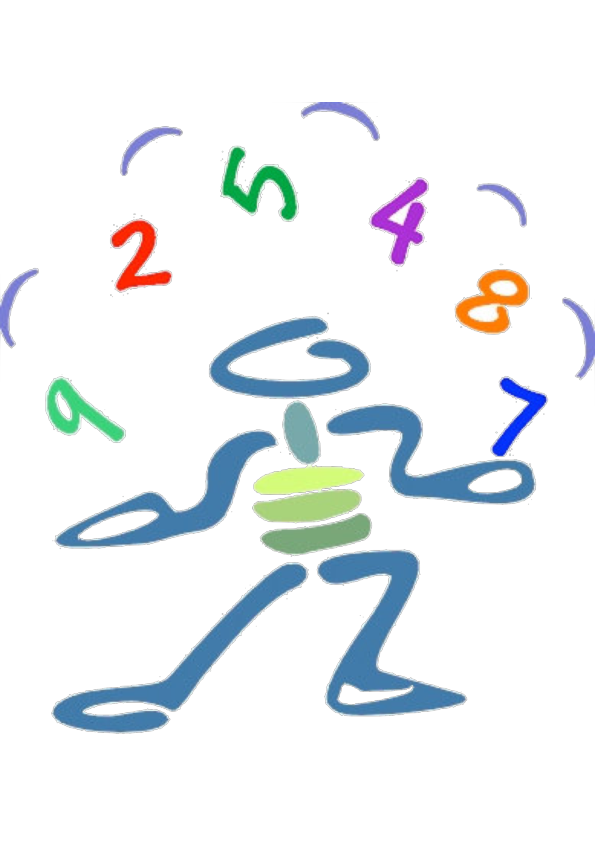
\includegraphics[width=8ex]{fig/01-problem}};
		\node[left=11ex of dle.south west, anchor=south, inner ysep=0, yshift=-1.2ex](dle-icon){
\includegraphics[width=8ex]{fig/01-cpu}};
	}},
	icon layers/.default={layers},
}

% Seite 1–10: Schichtenmodel ala Wosch + BST
\begin{frame}<1-2>[fragile]
\begin{tikzpicture}

	\pic{icon layers={layers}};
	\node<5->[at=(bse.east), anchor=east, inner sep=0, text width=9ex, font=\tiny\ttfamily, text=srared]{cli, sti, lidt\\~\\mov CR3, ...};

        \node [tooldesc, xshift=1ex,text=black] (mpe-bse) at ($(bse.north east)!0.5!(mpe.south east)+(right:1ex)$)
             {Teilinterpretation \mbox{(Betriebssystem)}};

        \node[tooldesc, above of=mpe-bse, onslide=<2->{rounded corners=0.5ex, fill=luhblue!30}](ase-mpe){Übersetzung (Assembler)\\Bindung (Linker)};
        \node[tooldesc, above of=ase-mpe, onslide=<2->{rounded corners=0.5ex,fill=luhblue, text=white}](pose-ase){Übersetzung (Compiler)};
        \node[tooldesc, below of=mpe-bse](bse-mae){Interpretation (Mikroprogramm)};
        \node[tooldesc, visible on=<1-3>, below of=bse-mae](mae-dle){Ausführung};

        \draw[dotted,ultra thick] (pose-ase.west) -- (pose-ase.west-|pose.west);

	\draw<2-> (HLL) node[tool=30, invisible on=<{3-}>]{gcc, clang};
	\draw<2-> (SYS) node[tool=40, invisible on=<{3-}>]{as, ld};
	\draw<2-> (BS) node[tool=50]{Linux};
	\draw<2-> (OPS) node[tool=60]{x86-64};
	\draw<2-> (mOPS) node[tool=70]{$\mu$-Ops};


	% VMs
	\tikzset{onslide=<6->{machine/.append style={fill opacity=1}}}
	\node[machine, anchor=south, at=(mpe)] (vm2) {VM 2};
	\node[machine, right=3ex of vm2] (vm3) {VM 3};
	\node[machine, left=3ex of vm2] (vm1) {VM 1};
	\path<4->[ultra thick, draw=srared, every to/.style={shorten <=-2pt}]
	($(vm1.north)!.5!(vm2.north)$) -- ($(vm1.south)!.5!(vm2.south)+(down:3ex)$)
		($(vm3.north)!.5!(vm2.north)$) -- ($(vm3.south)!.5!(vm2.south)+(down:3ex)$)
		;

	% Löcher in VMs (sharing)
		\node<6->[shared, at={($(vm1)!.5!(vm2)$)}, yshift=1ex]{shared};
		\node<6->[shared, at={($(vm2)!.5!(vm3)$)}, yshift=-3ex]{shared};


	\pgfresetboundingbox
	\useasboundingbox (dle-icon.west |- BBsouth.south) rectangle (mpe-bse.east |- SW.north);
\end{tikzpicture}
\end{frame}



\end{document}
% vim: filetype=tex
